%%%%%%%%%%%%%%%%%%%%%%%%%%%%%%%%%%%%%%%%%%%%%%%%%%%%%%%%%%%%%%%%%%%%%%%%%%%%%%%
%% LaTeX-Vorlage für Abschlussarbeiten                                       %%
%% (TH Köln -Campus Gummersbach, Fak. 10)                                    %%
%%                                                                           %%
%% Gemäß dem Merkblatt zur Anfertigung von Projekt-, Bachelor-, Master- und  %%
%% Diplomarbeiten der Fakultät 10 von Frau Prof. Dr. Halfmann &              %%
%% Herr Prof. Dr. Rühmann (Version vom 27.01.2008)                           %%
%%                                                                           %%                                                                            
%% Bitte sprechen Sie unbedingt mit Ihrer Betreuerin bzw. Ihrem Betreuer     %%
%% bezüglich der Ausgestaltung Ihrer Arbeit!                                 %%
%%                                                                           %%
%%                                                                           %%
%% MERKKASTEN IN DIESER VORLAGE:                                             %%
%% In dieser Vorlage finden Sie Merkkasten, die Ihnen Informationen          %%
%% zu bestimmten, formalen Aspekten geben. Sprechen Sie immer auch mit       %% 
%% Ihrer Betreuerin bzw. Ihrem Betreuer dazu an.                             %%                       
%% Für die eigene Verwendung der Vorlage entfernen oder kommentieren Sie die %%
%% Merkkasten. Die betreffenden Bereiche für die Merkkasten in der Vorlage   %%
%% sind wie folgt kommentiert: <MERKKASTEN> ... </MERKKASTEN>.               %%                            %%                                                                           %%
%%                                                                           %%
%% LIZENZ:                                                                   %%
%% Diese Vorlage darf nicht kommerziell verbreitet                           %%
%% werden. Eine nicht-kommerzielle Weitergabe ist                            %% 
%% gestattet.                                                                %%
%%                                                                           %%
%% Von Ludger Schönfeld, M. Sc.,
%% 2014-2017                            %%
%%%%%%%%%%%%%%%%%%%%%%%%%%%%%%%%%%%%%%%%%%%%%%%%%%%%%%%%%%%%%%%%%%%%%%%%%%%%%%%

%%%%%%%%%%%%%%%%%%%%%%%%%%%%%%%%%%%%%%%%%%%%%
%% HEADER                                  %%
%%%%%%%%%%%%%%%%%%%%%%%%%%%%%%%%%%%%%%%%%%%%%
\documentclass[a4paper,12pt,oneside]{article}
% Optionen:
% - a4paper => DIN A4-Format
% - 12pt    => Schriftgröße (weitere  
%              grundlegende Fontgrößen: 10pt, 11pt)
% - oneside => Einseitiger Druck

%% Verwendete Pakete:
\usepackage[ngerman]{babel} % für die deutsche Sprache
\usepackage{caption} % Für schönere Bildunterschriften
\usepackage[T1]{fontenc} % Schriftkodierung (Für Sonderzeichen u.a.)
\usepackage[utf8]{inputenc} % Für die direkte Eingabe von Umlauten im Editor u.a.
\usepackage{fancyhdr} % Für Kopf- und Fußzeilen
\usepackage{lscape} % Für Querformat

%% Schriften (Beispiele)
%% Weitere LaTeX-Schriften im "LaTeX Font Catalogue"
%% unter: http://www.tug.dk/FontCatalogue/.
%% ACHTUNG: Ggf. müssen Schriften noch installiert 
%% werden!

% Serifen-Schriften:
\usepackage{lmodern} % Schriftart "Latin Modern"
%\usepackage{garamond} % Schriftart "Garamond"

%Sans Serif-Schriften:
%\usepackage[scaled]{uarial}
%\usepackage[scaled]{helvet}
%%--------------
\usepackage[normalem]{ulem} % Für das Unterstreichen von Text z.B. mit \uline{}
\usepackage[left=3cm,right=2cm,top=1.5cm,bottom=1cm,
textheight=245mm,textwidth=160mm,includeheadfoot,headsep=1cm,
footskip=1cm,headheight=14.599pt]{geometry} % Einrichtung der Seite 

\usepackage{graphicx} % Zum Laden von Graphiken
% INFO: Graphiken einbinden
%
% \includegraphics[scale=1.00]{dateiname}
%
% => Ausgabeformat: PDF-Dokument:
%    Es können die folgenden (Graphik-)formate eingebunden
%    werden: .jpg, .png, .pdf, .mps
% 
% => Ausgabeformat: DVI/PS:
%    Folgende (Graphik-)formate werden unterstützt:
%    .eps, .ps, .bmp, .pict, .pntg
\usepackage{epstopdf}

% Pakete für Tabellen
\usepackage{tabularx} % Einfache Tabellen
\usepackage{longtable} % Tabellen als Gleitobjekte (für die Aufteilung bei langen 
 %Tabellen über mehrere Seiten)
\usepackage{multirow} % Für das Verbinden von Zeilen innerhalb einer Tabelle mit
 % \multirow{anzahl}{*}{Text}

% (Zusatz-)Pakete für Formeln
\usepackage{amsmath}
\usepackage{amsthm}
\usepackage{amsfonts}

\usepackage{setspace} % Paket zum Setzen des Zeilenabstandes
% INFO: Zeilenabstand setzen:
%
% Befehle:
% - \singlespacing  => 1-zeilig (Standard)
% - \onehalfspacing => 1,5-zeilig
% - \doublespacing  => 2-zeilig 
\onehalfspacing % Zeilenabstand auf 1,5-zeilig setzen

% Farbboxen (für die Merkkästen in dieser Vorlage):
\usepackage{tcolorbox}
\tcbset{colback=white,colframe=orange,
        fonttitle=\bfseries}
        
\usepackage{subfigure} 

\usepackage[colorlinks,pdfpagelabels,pdfstartview=FitH,
bookmarksopen=true,bookmarksnumbered=true,linkcolor=black,
plainpages=false,hypertexnames=false,citecolor=black]{hyperref} % Für Verlinkungen
% INFO: Verlinkungen mit dem hyperref-Paket:
%
% Die Angabe von URLs mit dem Befehl \url{} erlaubt einen
% gesonderten Umgang mit Weblinks. Denn die Links werden verlinkt.
% Auch erfolgt automatisch am Zeilenende ein Umbruch des Links.
% Es ist auch nicht erforderlich, Sonderzeichen in der URL manuell zu 
% entschärfen.
%
% TIPP: Sollte ein Umbuch bei einem Link nicht automatisch erfolgen, so kann
% das daran liegen, dass ein/mehrere Zeichen zusätzlich angegeben werden müssen,
% an dem der Link umbrochen werden kann.
% Dies kann mit folgendem Befehl erfolgen (Beispiel):
% \renewcommand*\UrlBreaks{\do-\do_}

% Das Paket "biblatex" für autom. 
% Literaturverzeichnisse:
%\usepackage{csquotes} % Für sprachangepasste Anführungszeichen
%\usepackage[backend=bibtex,style=alphabetic]  
%           {biblatex}
%\addbibresource{bib/literatur.bib}           

%%%%%%%%%%%%%%%%%%%%%%%%%%%%%%%%%%%%%%%%%%%%%
%% DOKUMENT                                %%
%%%%%%%%%%%%%%%%%%%%%%%%%%%%%%%%%%%%%%%%%%%%%
\begin{document}
  
  % Deckblatt
  \pagestyle{empty}
  \begin{titlepage}
    
\includegraphics[scale=1.00]{Sources/logo_TH-Koeln_CMYK_22pt}\\
    \begin{center}
      \Large
      Technische Hochschule Köln\\
      Fakultät für Informatik und Ingenieurwissenschaften\\
      \hrule\par\rule{0pt}{2cm} % Horizontale Trennlinie  mit 2 cm Abtand nach unten erzeugen
      \LARGE
      \textsc{Praxisprojekt WS18/19 - Dokumentation}\\
      \vspace{1cm} % Vertikaler Abstand von 1cm erzeugen
      \huge
      Entwicklung einer Objekterkennung für Regal-Systeme,
      mit Hilfe von Bildverarbeitung, in einem Neuronalen Netz\\
      \vspace{1 cm}
      \large
      Vorgelegt an der TH Köln\\
      Campus Gummersbach\\
      im Studiengang\\
      Medieninformatik\\ 
      \vspace{1.0cm}
      ausgearbeitet von:\\
      \textsc{Torben Krause}\\
      (Matrikelnummer: 11106885)\\
      \vspace{1.5cm}
      \begin{tabular}{ll} % Einfache Tabelle ohne Rahmen, mit 2 Spalten erzeugen
          \textbf{Prüfer/Betreuer:} & Prof. Dr. Martin Eisemann \\
      \end{tabular}
      \vspace{1.5cm}
      \\Gummersbach, 28.12.2018
    \end{center}    
  \end{titlepage}
  
  \newpage
  
  % Inhaltsverzeichnis
  \tableofcontents
  \newpage
  \listoffigures
 
  
  \newpage
  \pagestyle{plain}
  \pagenumbering{arabic}
  \setcounter{page}{1}
   
  
  \section{Motivation}
Das richtige Verwalten von Lebensmitteln, welche gekühlt im Kühlschrank aufbewahrt werden müssen, ist nicht immer leicht. Oft müssen schlecht gewordene Lebensmittel weggeschmissen werden, weil sie vergessen werden oder es fehlen Lebensmittel, welche gebraucht werden. Gerade in Haushalten mit mehreren Personen, wie zum Beispiel Familien oder Wohngemeinschaften, ist das Kühlschrankmanagement schwierig, da nicht jeder Bewohner weiß, welche Lebensmittel aus dem Kühlschrank genommen wurden und welche hineingelegt werden. Der häufigste Grund ist dabei die unzureichende Kommunikation unter den Bewohnern. Aus diesem Grund werden schnell verderbende Lebensmittel leicht vergessen oder Produkte durch fehlerhafte Absprache mehrfach oder nicht gekauft. \\ Eine Idee um dieses Problem zu lösen ist den Kühlschrankinhalt mithilfe einer Kamera, welche im Inneren des Kühlschranks angebracht ist, aufzuzeichnen und die enthaltenden Lebensmittel mit einem neuronalen Netz zu klassifizieren. Aus den Ergebnissen der Analyse wird nun eine Produktliste vom Inneren des Kühlschranks erstellt und anschließend in einer Datenbank gespeichert. Über eine mobile Anwendung können die erhobenen Daten dem Benutzer zur Verfügung gestellt werden.
  
  \subsection{Zielsetzung} 
Ziel dieses Projektes ist die Entwicklung eines künstlichen neuronalen Netzes, welches mehrere vordefinierte Klassen zuverlässig erkennt und zuordnen kann. Das Netz soll außerdem so konzipiert werden, das Produkte unabhängig ihrer Position im Bild erkannt werden können. Desweiteren soll das neuronale Netz auch mit leicht verdeckten Objekten zurecht kommen. Ein optionales Ziel, welches ebenfalls erstrebenswert ist, ist eine Unempfindlichkeit gegenüber Licht- und Bildqualitätsverhältnissen.  ????????? Soll dieser Satz raus????

\newpage
	
  \subsection{Anforderungen}
In diesem Kapitel sollen die Anforderungen an das zu entwickelnde künstliche neuronales Netz, mit Hilfe der Anforderungsschablonen von 'Die SOPHISTen'[QUELLE] definiert werden. 
  
  \subsubsection{Funktionale Anforderungen}
  
  \begin{itemize}
\item Das System muss fähig sein Bilder zu verarbeiten. 
\item Das System muss fähig sein die trainierten Klassen zu erkennen und einzuordnen.
\item Das System soll fähig sein mehrere Objekte auf einem Bild gleichzeitig zu erkennen und deren Position festzustellen.
  \end{itemize}  
	
  \subsubsection{Organisationale Anforderungen}
  
 \begin{itemize}
\item Das System wird so gestaltet sein, dass die existierenden Klassen unkompliziert erweitert werden können.
\item Das System wird so gestaltet sein, dass es mit wenig Aufwand betrieben werden kann.
\item Das System soll so gestaltet sein, dass es einfach auf ein Endgerät transferiert werden kann.
\item Die Installation benötigter Module soll für den Benutzer so einfach wie möglich gemacht werden.
  \end{itemize}
  
  \subsubsection{Qualitative Anforderungen}
  
 \begin{itemize}
\item Das zu trainierende Netz muss eine möglichst hohe Genauigkeit aufweisen. 
\item Das zu entwickelnde Netz soll auf den aktuellen Plattformen arbeiten und neue Technologien unterstützen.
\item Das System soll so ausgelegt werden, dass die Geschwindigkeit der Objekterkennung möglichst hoch ist.
\item Das System soll fähig sein leicht verdeckte Objekte richtig zu identifizieren.
\item Das System soll fähig sein bei schlechten Bildverhältnissen gute Ergebnisse zu liefern.
  \end{itemize}  
  
  \section{Künstliche Neuronale Netze}  
Die Bezeichnung \"neuronale Netze\" kommt aus der Biologie und beschreibt die Funktionsweise des menschlichen Gehirns. Das Gehirn eines Menschen besteht aus ungefähr $10^{11}$ Nervenzellen[QUELLE], den so genannten Neuronen. Diese sind untereinander verbunden und tauschen Informationen aus. Wird eine bestimmte Reizschwelle überschritten, werden Signale an das nächste Neuron weitergegeben. Ein neuronales Netz kann somit als eine Verbindung aus vielen Nervenzellen bezeichnet werden, welches Informationen verarbeitet und weiterleitet. Das neuronale Netz ist unter anderem für das menschliche Lernen zuständig. 
\\
\\
Ein künstliches neuronales Netz ist dementsprechend eine Nachahmung eines menschlichen Gehirns, welches auf Grundlage mathematischer Formeln arbeitet. Auf die verwendeten Formeln, wird in dieser Arbeit nicht eingegangen, eher soll die Funktionsweise von künstlichen neuronalen Netzen erläutert werden. Künstliche Neuronale Netze (KNN) stellen einen Bestandteil des maschinellen Lernens dar. Oft werden KNN für die Klassifizierung von Datensätzen (Bildern, Statistiken, Profile in sozialen Netzwerken) verwendet. Das Ergebnis der Klassifikation ist eine Zugehörigkeitswahrscheinlichkeit der Eingabedaten zu den definierten Klassen.
\\
\\
\begin{figure}
	[h]
	\centering
	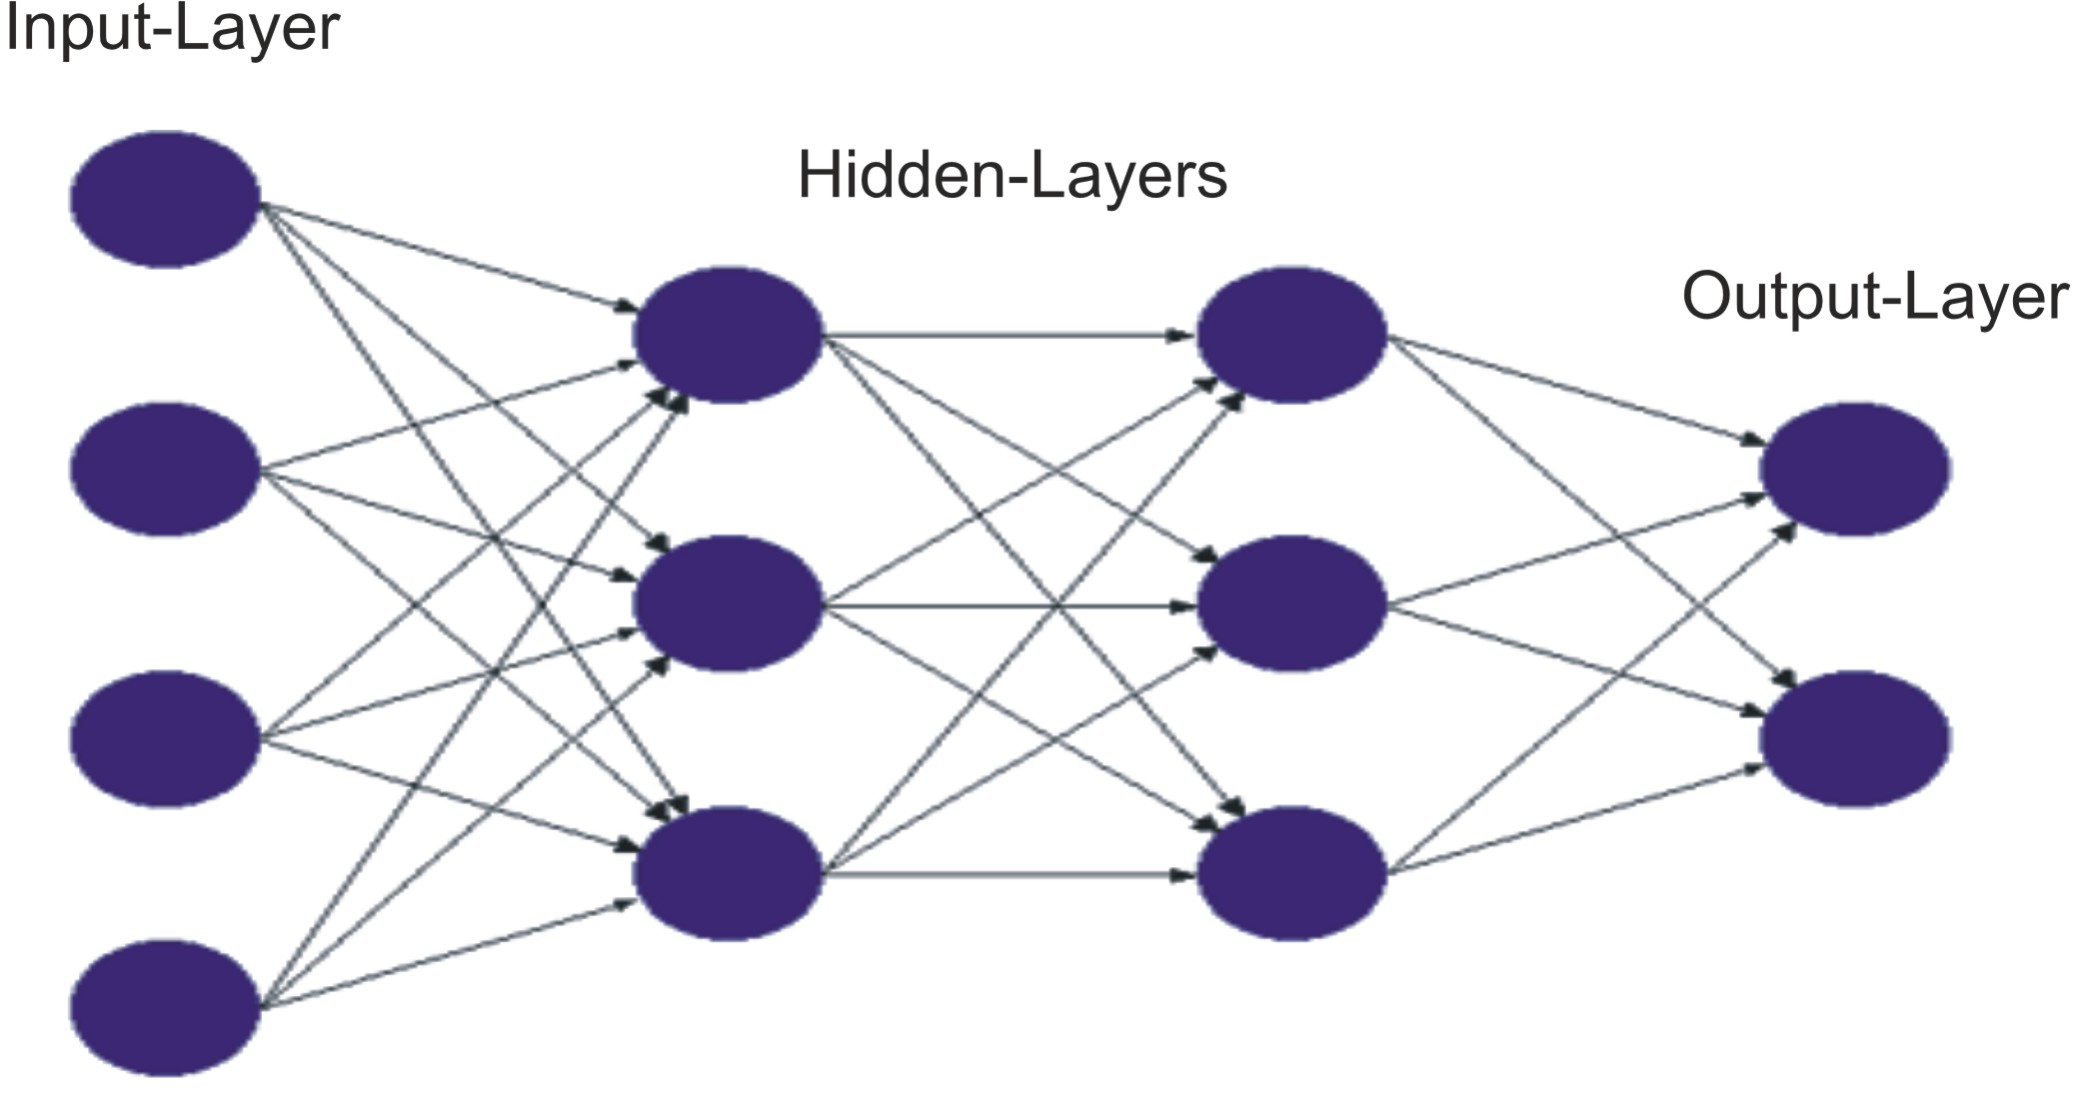
\includegraphics[scale=0.5]{Sources/nnet.png}
		\caption{Schematischer Aufbau eines künstlichen neuronalen Netzes [QUELLE] }
	\label{img:KNN}
\end{figure}
\\
\\
Der Aufbau eines künstlichen neuronalen Netzes kann grundsätzlich in drei Schichten aufgeteilt werden (Abbildung \ref{img:KNN}). Die erste Schicht ist der \"Input Layer\". Dieser \"Layer\" bekommt alle Eingangsdaten von einem Bild. Jeder Pixel auf dem Bild wird mit einem Neuron verbunden, welche sich in der Gewichtung und dem Schwellwert unterscheiden können. Wird der Schwellwert überschritten, gibt das Neuron die verarbeiteten Informationen an die nächste Schicht weiter. Die zweite Schicht besteht aus einem oder mehreren \"Hidden Layer\". Jeder \"Layer\" ist in dieser Schicht auf verschiedene Merkmale trainiert. Anfangs werden nur grobe Strukturen erkannt, wie beispielsweise Geraden oder Kanten. Diese Strukturen werden detaillierter, desto mehr \"Layer\" durchlaufen wurden. Die dritte Schicht besteht aus dem \"Output Layer\". Die Muster die in den vorherigen Layern erkannt und zusammengesetzt wurden, vergleicht der \"Output Layer\" mit den trainierten Klassen und gibt eine prozentuale Wahrscheinlichkeit aus, welche Klassen in dem Bild enthalten sind.


  \subsection{Convolutional Neural Network}
Anders als bei einem KNN, welches auf Grundlage des Menschlichen Gehirns entworfen wurde, orientiert sich ein \"Convolutional Neural Network\" (CNN) an dem Konzept des menschlichen Sehens. Dabei werden maschinell, kleine Bereiche visueller Informationen so simuliert, als wären sie benachbarte Sehnerven im Auge[QUELLE]. Gerade für die Verarbeitung von Bilddaten werden häufig \"Convolutional Neural Networks\" eingesetzt. Voraussetzung für ein CNN ist die Darstellung und Anordnung der Datenpunkte. Diese müssen eine matrixartige Anordnung von Werten haben, wie beispielsweise Pixel.
\\
\\
Bei einem \"Convolutional Layer\" (Abbildung \ref{img:CNN}), oder auch im Deutschen Faltungsschicht, werden über die Pixel des Eingabebildes eine Schablone gelegt. Diese wird je nach Bildgröße, mehrere male Horizontal wie auch Vertikal verschoben. Diese Layer haben meist eine ungerade quadratische Abmessung (3x3, 5x5, 7x7). Die frühen schichten bilden zunächst ein Skalarprodukt der betroffenen Pixel und können dadurch grobe kanten erkennen. Jeder Layer ist dabei auf eine bestimmte Art von Mustern trainiert. Je mehr Layer durchlaufen, desto genauer werden die Muster welche das neuronale Netz erkennt und umso mehr wird das Eingabebild runter skaliert.

\begin{figure}
    [h]
	\centering
	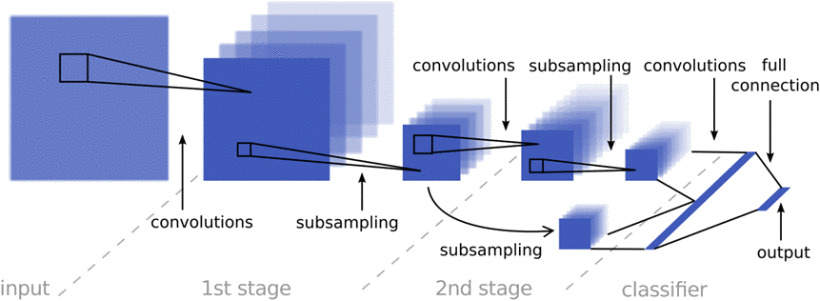
\includegraphics[scale=1.5]{Sources/cnn.png}
		\caption{Funktionsweise eines Convolutional Neural Network [QUELLE]}
	\label{img:CNN}
\end{figure}

Der \"Pooling Layer\" (Abbildung \ref{img:CNN}) funktioniert ähnlich wie der \"Convolutional Layer\". Auch bei dieser Methode wird eine Schablone über die Pixel des Bildes gelegt und Horizontal wie auch Vertikal verschoben. Hierbei werden die Farbwerte der beteiligten Pixel verarbeitet. Es kann entweder der höchste Farbwert eines Pixels übernommen, oder der durchschnittliche Farbwert berechnet werden. Die letzten Schichten des Netzes bestehen aus \"Fully Connected Layer\" welche den normalen Aufbau eines künstlichen neuronalen Netzes darstellt. Das bedeutet, alle Ausgaben werden wie beim KNN mit jedem Neuron verbunden. Die letzte Schicht übergibt seine Ausgaben an den Output Layer, welcher die Wahrscheinlichkeiten der Objekte berechnet[QUELLE].
  
  \subsection{Abwägung von Neuronalen Netzen} 
Für das Entwickeln eines neuen neuronalen Netzes wird eine hohe Anzahl an Trainingsdaten sowie viel Rechenleistung benötigt. Bestehende Netze wurden mit mehreren 100 Tausend Bilden, mehrere Tage, bis Wochen lang trainiert. Eine andere Möglichkeit besteht darin, frei verfügbar trainierte Netze zu verwenden. Diese Netze haben für ihre bis zu 80 Klassen eine Genauigkeit von durchschnittlich 90 Prozent oder eine mAP (Mean Average Precision) von 30. Einige dieser trainierten Netze werden von Unternehmen als Open-Source zur Verfügung gestellt.
\\
\\
Um ein eigenes Netz mit einer annähernd hohen Genauigkeit zu erreichen ist in der Hinsicht auf die eigenen Ressourcen schwierig. Aus diesem Grund, soll für das Projekt ein bestehendes Neuronales ausgewählt werden welches mit eigenen Klassen und Trainingsdaten trainiert wird. Die Kriterien für das ausgewählte Netz, sind zum einen eine hohe Genauigkeit und eine moderate Geschwindigkeit haben mit der das spätere System effizient arbeiten kann. Der wichtige Aspekt ist die Genauigkeit und Verlässlichkeit der Prognosen. Weitere Anforderungen wurden in den vorherigen Kapiteln bereits aufgestellt.
\\
\\
In der folgenden Abwägung, wurden einige verfügbare Netze aufgeführt, die für Tensorflow zur Verfügung gestellt werden. Dabei werden die aufgeführten Modelle in Genauigkeit und Geschwindigkeit verglichen.
 
  \subsubsection{Auswahl des Netzes} 
In Hinsicht auf Trainierte Netze bietet \"Tensorflow\" einige Möglichkeiten an. Hierbei handelt es sich um die \"Tensorflow detection model zoo\"[QUELLE] welche mit verschiedensten Datensätzen und Durchläufen trainiert wurden. Die Datensätze die verwendet wurden sind unter anderem das COCO dataset, das Kitti dataset, das Open Images dataset, das AVA v2.1 dataset und das iNaturalist Species Detection Dataset. Die COCO-Models bieten das größte Spektrum an Netzen. Bei dem COCO Datenset handelt es sich um 'Common Objects In Context' und beinhaltet rund 330 Tausend Bilder, welche über 1.5 Millionen schichten in 90 Klassen trainiert wurden. Da es sich um häufige auftretende Objekte in einer realen Umgebung handelt, sind die Modelle gut für unser vorhaben geeignet. In der folgenden Tabelle, wurden ein paar dieser Modelle ausgesucht und verglichen.
\\
\\

\begin{table}
[h]
\begin{tabular}{|l|c|c|c|}
 
Modell Name & Geschwindigkeit & COCO mAP & Ausgabe\\
 & & & \\
faster\_rcnn\_inception\_v2\_coco & 58 ms & 28 & Boxen\\
 & & & \\
faster\_rcnn\_resnet50\_coco & 89 ms & 30 & Boxen\\
 & & & \\
rfcn\_resnet101\_coco & 92 ms & 30 & Boxen\\
 & & & \\
faster\_rcnn\_resnet101\_coco & 106 ms & 32 & Boxen\\
 & & & \\
ssd\_mobilenet\_v1\_fpn\_coco & 53 ms & 32 & Boxen\\
 & & & \\
ssd\_resnet\_50\_fpn\_coco & 76 ms & 35 & Boxen

\vspace{0.5 cm}
 
\end{tabular}
\caption{Trainierte Modelle auf dem COCO Dataset [QUELLE]}
\end{table}


In der Tabelle, werden 6 mögliche Modelle aufgeführt. Beschrieben werden diese durch eine Geschwindigkeit in welcher das Neuronale Netz im durchschnitt arbeitet, einer Genauigkeit und eines Ausgabetyps. Die zweite Spalte, COCO mAP gibt die mittlere durchschnittliche Genauigkeit an, mit welcher es Objekte erkennt. Berechnet wird diese durch die Genauigkeit der richtigen Ergebnisse im Vergleich auf alle ausgeführten Durchläufe des Systems. In der Letzten spalte wird die Ausgabeform beschrieben. Hierbei kann zwischen Boxen und Masken unterschieden werden. Dabei wird je nach Ausgabetyp entweder ein viereckiger Kasten (Abbildung \ref{img:Boxes}) um das object erstellt, oder es wird eine Maske (Abbildung \ref{img:Mask}) über dieses gezogen.

%einbinden einer Grafik 
\begin{figure} 
	[h]
	\centering
    \subfigure[Makierung durch Maskierung]{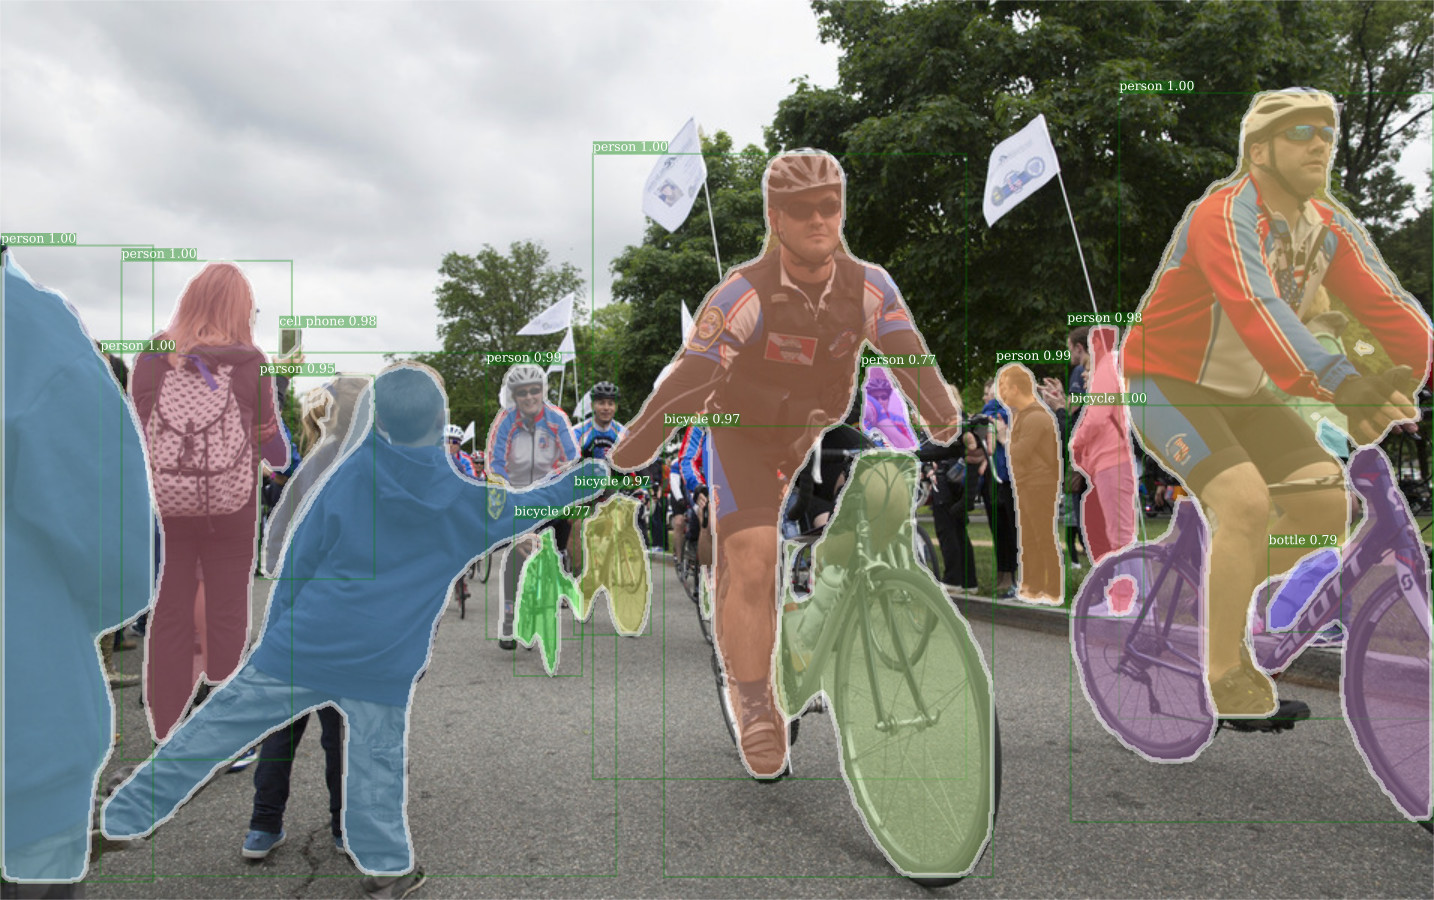
\includegraphics[width=0.39\textwidth]{Sources/sample.jpg}}
    \label{img:Mask} 
    \subfigure[Makierung durch Kästen]{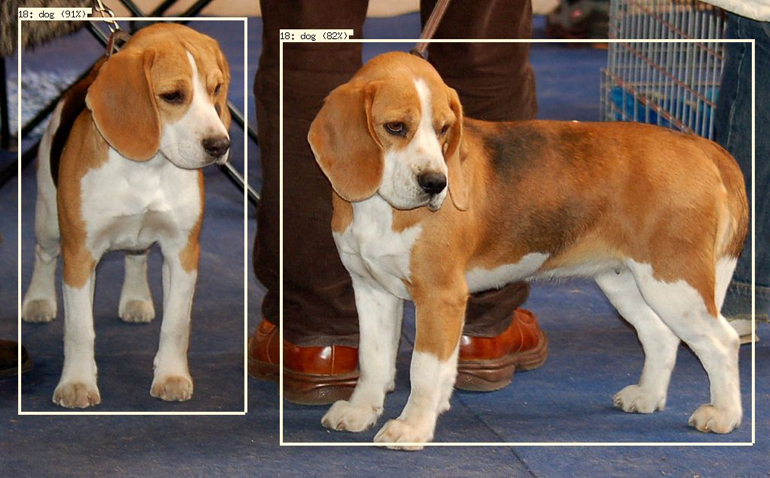
\includegraphics[width=0.39\textwidth]{Sources/boxes.jpg}}
    \label{img:Boxes} 
\caption{Ausgaben von Neuronalen Netzen [QUELLE]} 
\end{figure} 

\newpage

Bei dem Vergleich der Aufgezählten Modellen fällt auf, das alle eine ähnliche Genauigkeit aufweisen und sich leicht unterscheiden. In der Geschwindigkeit jedoch werden die Unterschiede erkennbar größer. Durch die hohe Geschwindigkeit und vergleichsweise hohe Genauigkeit, wird vorerst das faster\_rcnn\_inception\_v2\_coco Modell getestet, und ausgewertet.
\\

Das ausgewählte Modell wurde für Testzwecke mit 6 Klassen um-trainiert. Die Klassen bestanden aus einem Skart-kartenset von Neun bis Ass [QUELLE]. Rund Fünf Stunden wurde das Netz trainiert, und hat dabei 60 tausend Testdurchläufe absolviert. Eine Überprüfung des Netzes hat eine Genauigkeit von 97 bis 99 Prozent ergeben. Auch Tests ergeben das die Erkennung fehlerfrei funktioniert. Das Testbild (Abbildung \ref{img:Kartenset} zeigt, das alle Karten mit einer hohen Wahrscheinlichkeit identifiziert werden konnten.
\\
\begin{figure}
    [h]
	\centering
	\includegraphics[scale=0.5]{Sources/kartenset.png}
	\caption{Analysiertes Bild, durch das Testnetz [QUELLE]}
	\label{img:Kartenset}
\end{figure}
\\
Das erfolgreiche Training und testen des Netzes hat die Verwendung des Ausgewählten Modells bestärkt. Die Vorgehensweise sieht in den weiteren Schritten eine Definition und Festlegung der Trainings-Daten für das benötigte neuronale Netz. 

\newpage

  \section{Durchführung}
In diesem Kapitel der Dokumentation, wird die Praktische Durchführung beschrieben und Entscheidungen aufgeführt. Dabei werden die verwendeten Frameworks und die Entwicklungsumgebung aufgezeigt und erläutert. Im weiteren geht es um das festlegen der Klassen für das Netz und die anschließende Durchführung.

\subsection{Entwicklungsumgebung}
Um ein bestehendes neuronales Netz neu zu trainieren werden neben dem dem Neuronalen Netz weitere Frameworks sowie eine Entwicklungsumgebung benötigt. In den kommenden Unterpunkten wird die Entwicklungsumgebung sowie alle benötigten Bibliotheken aufgeführt. 

  \subsubsection{Verwendete Hardware Konfiguration}
Das Netz wurde auf einem Windows 8.1 Betriebssystem trainiert. Berechnet wurden die Trainingsschritte von einer Nvidia GeForce GTX 980 GPU mit 4GB VRAM, einer Intel Core i5 CPU und 16GB RAM (Arbeitsspeicher). Für einen Trainingsschritt, mit dem ausgewählten Netz, benötigt die Grafikkarte durchschnittlich 250ms. Im Vergleich hat die CPU 2 Sekunden pro Schritt benötigt. Die Grafikkarte arbeitet somit 8 mal schneller durch den Vorteil mit Matrixmultiplikationen und soll für das Training verwendet werden.

  \subsubsection{Anaconda python}
Das verwendete CNN wurde in der Programmiersprache Python erstellt, weswegen wir zum um-trainieren mit Python arbeiten. Des weiteren bietet Python eine Vielzahl an verfügbaren Bibliotheken welche wir benötigen. Anaconda ist eine \"Open-Source-Distribution\" für die Programmiersprache Python. Mit dieser können wir gleichzeitig mehrere Versionen von Python generieren und die notwendigen Bibliotheken installieren. Anaconda bietet den Vorteil einfach zwischen den verschieden Python Versionen wechseln zu können \\
In diesem Projekt wurde mit der Python version 3.6.7 gearbeitet.

  \begin{itemize}
	\item Installation von Python 3.6.7: conda create -n <Name> python=3.6.7
  \end{itemize}
  
  \subsection{Frameworks}
Um das Künstliche neuronale Netz zu trainieren, wird ein Framework und mehrere Programm-Bibliotheken benötigt. Die Auswahl wird im folgenden aufgezählt und kurz erläutert.
 
  \subsubsection{Tensorflow}
Bei Tensorflow handelt es sich um eine Plattform unabhängige Programmbibliothek unter Open-Source-Lizenz, die sich für Aufgaben rund um maschinelles Lernen und Künstliche Intelligenz (KI) einsetzen lässt. Ursprünglich entwickelte Google die Software für den internen Bedarf. Das Framework bietet vielfältige Einsatzmöglichkeiten und gestattet es, lernende neuronale Netze zu erstellen und diese zu verändern. Es zeichnet sich durch seine gute Skalierbarkeit aus und ist auf unterschiedlichen Systemen vom Smartphone bis zu Clustern mit vielen Servern betreibbar. Außerdem verweist Google auf verschiedenste trainierte Modelle welche für das Projekt verwendet werden. Tensorflow kann auf allen CPU's betrieben werden, oder mit Nvidia Grafikkarten, welche CUDA unterstützen.

  \begin{itemize}
\item Installation in Python: pip install --upgrade gpu-tensorflow
  \end{itemize}
  
Verwendet wird zusätzlich die API von Tensorflow (Models) für die Objekterkennung. In dieser wird eine Grundstruktur für das Trainieren eines CNN zur Verfügung gestellt, welche man je nach Verwendungszweck anpassen kann.
  
  \subsubsection{Benötigte Bibliotheken}
Für das Arbeiten mit Tensorflow und CNN's benötigt man einige spezielle Python Bibliotheken. Diese werden im folgenden aufgeführt und erläutert. Die Installation geschieht hier über den \"Package Installer\" von Python.
\\
 
\textbf{Pillow}\\\\
Pillow ist eine \"Imaging Library\" für Python. Diese Bibliothek wird dafür genutzt um Bilddateien zu öffnen, verändern und speichern zu können. Pillow benötigen wir, um in unserem Künstlichen neuronalen Netz mit Bildern und Videos arbeiten zu können.

  \begin{itemize}
\item Installation in Python: pip install --upgrade pillow
  \end{itemize}

\textbf{lxml}\\\\ 
lxml ist eine Weiterführung der XML Sprache für Python. lxml erweitert dabei den Elementebaum von XML stark. Verwendet wird lxml dafür, um die Markierungen von Klassen und deren Positionen auszulesen, damit diese umgewandelt werden können. Durch die Arbeit mit Elementbäumen werden nur die benötigten Informationen herausgefiltert, wodurch wir eine schnellere Ausführung und bessere Arbeitszeiten erreichen.
  
  \begin{itemize}
\item Installation in Python: pip install --upgrade lxml
  \end{itemize}
  
  
\textbf{Cython}\\\\
Python ist im vergleich zu C eine recht langsame Programmiersprache, was die Ausführungzeit des Programmcodes wesentlich erhöht. Cython ist eine Programmbibliothek und auch Programmiersprache, welche die wesentlich langsame Programmiersprache Python erweitert und in der Ausführung beschleunigt. Dabei wird Python-Code in C kompiliert oder es kann externer code von C, eingebunden werden um ihn für die Ausführung zu nutzen. Das hat den Vorteil, das die Geschwindigkeit des Programms erhöht wird. Gerade für das Trainieren künstlicher neuronaler Netze, wird viel Rechenleistung benötigt. Das führt zu einer hohen Ausführungszeit des Programms. Um eine bessere Performance erreichen zu können greifen wir auf Cython zurück.

  \begin{itemize}
\item Installation in Python: pip install --upgrade Cython
  \end{itemize}

\textbf{Jupyter}\\\\
Jupyter oder auch \"Jupyter Notebook\" ist eine open-source Web Applikation die es ermöglicht Dokumente welche Live Code, Abbildungen oder Text beinhalten zu teilen. Dabei kann man den Inhalt der Dateien im Browser aufrufen und ausführen. Verwendet wird diese Bibliothek, um die Lauffähigkeit des Neuronalen Netzes zu überprüfen.  

\begin{itemize}
\item Installation in Python: pip install --upgrade jupyter
  \end{itemize}
  
\textbf{matplotlib}\\\\
Die Programmbibliothek matplotlib ermöglicht es mit python, mathematische Darstellungen in der Python-Konsole oder im Code integriert anzufertigen und Visuell auszugeben.
Matplotlib wird zum einen dafür verwendet die Erkennung, eines Objektes, auf einem Bild, an der jeweiligen Position anzuzeigen und zu beschreiben.

  \begin{itemize}
\item Installation in Python: pip install --upgrade matplotlib
  \end{itemize}
  
\textbf{Pandas}\\\\
Pandas ist eine Programmbibliothek von Python. Der Name stammt von \"Paneldata\", was eine Bezeichnung von Datensätzen ist. Diese Bibliothek kann für die selektierung und Inditzierung von Daten verwendet werden. In dem künstlichen neuronalen Netz, wird pandas unter anderem für die Erhebung der XML Dateien der Trainingsdaten verwendet.

  \begin{itemize}
\item Installation in Python: pip install --upgrade pandas
  \end{itemize}
  
\textbf{opencv-python}\\\\
OpenCV steht für „Open Source Computer Vision Library“ und ist eine freie Programmbibliothek für maschinelles Sehen. Dadurch, das dass zu entwickelnde CNN auf Basis von visuellen Daten arbeiten soll, welche mehr als ein Objekt gleichzeitig beinhalten kann, benötigen wir eine Aufteilung von Bildbereichen. Weitere Einsatzbereiche entstehen dann, wenn Beispielsweise die Helligkeit des Bildes nicht ausreicht. Hierbei kann die Helligkeit künstlich angepasst werden.

  \begin{itemize}
\item Installation in Python: pip install --upgrade opencv-python
  \end{itemize}
  
  \subsection{Trainingsdaten Generieren} 
Zu beginn ist ein un-trainiertes neuronales Netz noch "Dumm", da es bis zu diesem Zeitpunkt noch kein wissen darüber hat, welche Objekte es erkennen soll und welche Eigenschaften diese haben. Damit das zu entwickelnde Neuronale Netz weiß was es erkennen und klassifizieren soll, müssen zunächst Trainings und Testdaten generiert werden. Für das Training werden optimaler weise mehrere Tausend Trainings- und Testbilder benötigt, damit eine möglichst hohe Genauigkeit erreicht werden kann. Auch die Trainingsphase dauert in der Ausführung einige Stunden. 
\\
\\
Wie in der Auswahl des Neuronalen Netz bereits beschrieben wird wegen der begrenzten Zeitressource ein trainiertes Netz von COCO verwendet. der Vorteil bei der Verwendung eines bereits trainierten Netzes besteht darin, das die Gewichtungen der frühen Layer gut eingestellt sind und diese nicht verändert werden müssen. Lediglich die obersten Layer sollen mit den eigenen Daten um-trainiert werden. Dadurch das die Gewichtungen der untersten Layer trainiert sind werden weniger Trainings- und Testdaten benötigt, um eine hohe Genauigkeit des Neuronalen Netzes zu erreichen.

  \subsubsection{Funktionsweise}
Wie gerade schon angeschnitten, bekommen bei Netzen welche neu trainiert werden jedes Neuron zunächst ein zufälliges Anfangs-Gewicht und Schwellwert. Beim starten der Trainingsphase werden Daten in das Netz eingeführt. Jedes Neuron verarbeiten nun alle Eingangssignale mit der zugewiesenen Gewichtung und geben die Ergebnisse an das nächste Neuron weiter. 
\\
\\
Im Output-Layer wird nun das Ergebnis der Berechnungen ermittelt. Das Ergebnis des Netzes wird mit der Tatsächlichen Bezeichnung des Objektes verglichen. Lag das Netz bei der Bestimmung falsch wird zunächst der entstandene Fehler Berechnet und die Neuronen werden dementsprechend angepasst. Dabei werden die Gewichtungen der Neuronen so stark verändert je mehr Einfluss diese auf das resultierende Ergebnis hatten. Dieser Vorgang wird nun viele male wiederholt. Das ist die kurze Fassung, wie ein Künstliches Neuronales Netz lernt. 
  
  \subsubsection{Auswahl der Klassen} 
Bei der Auswahl der Klassen wurde darauf geachtet, die Genauigkeit des Netzes zu erkennen, indem Klassen ausgewählt werden, welch eine gewisse Ähnlichkeit aufweisen jedoch unterschiedliche Bezeichnungen haben. Beispiele sind hier Flaschen, Tetra Packs oder auch Schachteln.

  \vspace{0.5 cm}

  \begin{itemize}
  
  \item ID: 1 Name: 'Bier, Flasche'

  \item ID: 2 Name: 'Wasser, Flasche'

  \item ID: 3 Name: 'Milch, Packung'

  \item ID: 4 Name: 'Orangensaft, Packung'

  \item ID: 5 Name: 'Brunch, Aufstrich'

  \item ID: 6 Name: 'Margarine, Aufstrich'
  
  \end{itemize}
    
  
  \newpage
  
  \subsection{Trainieren}
Damit das zu entwickelnde Netz für die ausgewählten Klassen verwendet werden kann, muss ein großer Datensatz generiert werden. Wie im obrigen Abschnitt beschrieben, werden Klassen ausgewählt, welche eine gewisse Ähnlichkeit aufweisen. Dadurch soll überprüft werden, ob das neuronale Netz auch Objekte mit nur kleinen Unterschieden auseinanderhalten kann.\\
Als Testobjekte wurden zwei Tetra Packs, zwei Flaschen und zwei Aufstriche verwendet. Die Einteilung der Klassen wird in der folgenden Tabelle gezeigt.
\\
\\

\begin{table}
[h]
\centering
\caption{Ausgewählte Klassen und Struktur}
\begin{tabular}{|c|l|c|}
 
   Klasse   &   Bezeichnung   &   Bereich   \\
 & & \\
   1   &   Milch - Packung   &   1-99   \\
 & & \\
   2   &   Orangensaft - Packung   &   100-199   \\
 & & \\
   3   &   Wasser - Flasche   &   200-299   \\
 & & \\
   4   &   Bier - Flasche   &   300-399   \\
 & & \\
   5   &   Brunch - Aufstrich   &   400-499   \\
 & & \\
   6   &   Margarine   &   500-599   \\
 & & \\
   7   &   Gemischt   &   600-699
 
\end{tabular}
\end{table}

\vspace{1 cm}

Zunächst müssen Testdaten in Form von Bildern generiert werden, dafür wurden zum einen, Bilder von Online-Suchmaschinen, je nach Verwendbarkeit für das Netz heruntergeladen. Dabei sollte das Bild eine Größe von 200 KB nicht übersteigen, damit das Training erfolgreich verläuft und nicht zusätzlich mehr Zeit benötigt. Des weiteren wurden Objekte der aufgeführten Klassen, in verschiedensten Winkeln und Lichtverhältnissen Fotografiert. Die aufgenommenen Bilder übersteigen mit 3-5 MB die maximale Größe der Testdaten. Aus diesem Grund, wurden die Bilder mit einem Programm um den Faktor 0.2 verkleinert. Verwendet wird für die Komprimierung ein in Python geschriebenes Programm (reziser.py).\\
\\
Damit die API von Tensorflow weiß, welche Klassen auf dem Bild zu sehen sind und wo sich diese im Bild befinden, müssen die Bilder gelabelt werden, hierfür wurde das Programm labelImg.py verwendet. Beim labeln werden die zu klassifiezierenden Objekte auf dem Bild mit den Positionsdaten und Bezeichnung markiert und in einer XML Datei abgespeichert. Nach dem markieren werden Die Daten in Trainings und Testdaten aufgeteilt. 80 Prozent kommen in den Trainingsordner und 20 Prozent in den Testordner. Für die Durchführung des Trainings werden die Informationen der einzelnen XML Dateien, in zwei CSV Dateien zusammengefasst. Diese Dateien beinhalten Tabellen in denen alle Notwendigen Informationen zu den Bildern aufgeführt werden. Verwendet wird dafür das Programm xml\_to\_csv.py.\\
\\
Nachdem alle Bilddaten gelabelt wurden und die CSV Dateien für die Trainings- und Testdaten erstellt wurden, kann das Training beginnen. Zusätzlich zu den Traningsdaten wird eine  Labelmap (labelmap.pbtxt) benötigt in welcher die ausgewählten Klassen eingetragen sind ???Was sind die Ausgewählten KLassen, bzw was meinst du mit ausgewählt???. Außerdem brauchen wir die konfigurations Datei des verwendeten Netzes (faster\_rcnn\_inception\_v2\_coco). Das Training wird mit Ausführung des training.py Programms gestartet. Ab diesem Zeitpunkt, benötigt das Training viel Zeit.\\\\
Zusätzlich Parameter: \\
\textbf{--logtostderr}\\
\textbf{--train\_dir=training/}\\
Dieser Parameter gibt den Pfad zum Ordner an in welchem die Trainingsergebnisse Gespeichert werden sollen.\\
\textbf{--pipeline\_config\_path=training/faster\_rcnn\_inception\_v2\_coco.config}\\
Dieser Parameter gibt den Pfad zu der benötigten config Datei an\\\\
\\
Damit die Ergebnisse so gut wie möglich ausfallen, wird das Netz ca. 10 Stunden, mit der in Kapitel? beschriebenen Konfiguration Trainiert. Dabei schafft das Programm 200.000 Trainings- und Testdurchläufe und ist kurz vor Abschluss der Trainingsphase bei einem durchschnittlichen 'loss' von 0,03. Alle 5 Minuten werden die Zwischenstände gespeichert. Aus dem letzten Standpunkt des Trainings wird mit hilfe des export\_inference\_graph.py  ein Sogenannter 'frozen inference graph' generiert, welcher unser Künstliches neuronales Netz darstellt.\\\\
Mitgegebenen Parameter:\\
\textbf{--input\_type image\_tensor}\\
\textbf{--pipeline\_config\_path legacy/training/faster\_rcnn\_inception\_v2\_coco.config}\\
Gibt den Pfad zur config Datei an.\\
\textbf{--trained\_checkpoint\_prefix legacy/training/model.ckpt-XXXX}\\
Gibt den Pfad zur letzten Speicherstand des Trainings an.\\
\textbf{--output\_directory inference\_graph}\\
Bestimmt den Ort an welchen der Graph exportiert wird.\\\\

Ab diesem Zwischenstand, kann das Neuronale Netz für die Objekterkennung verwendet werden.
  
\newpage

\section{Testergebnisse}
In diesem Kapitel soll die Zuverlässigkeit sowie Geschwindigkeit, des neuronalen Netzes geprüft und ausgewertet werden. Dazu wird das Netz mit ungelabelten Bildern getestet, wobei nur Testbilder verwendet werden, welche nicht im Trainings- und Testdatensatz vorhanden waren. Es soll sichergestellt werden, dass das Netz die Objekte nicht durch das Training kennt. Anschließend wird überprüft wie zuverlässig das Netz ist und ob es alle Objekte erkannt hat. 
\\
Tensorflow bietet mit dem Tool Tensorboard die Möglichkeit den fortschritt des Trainings grafisch darzustellen. In der folgenden Grafik wird der auftretende 'Loss' in Verhältnis zu der Trainingszeit gestellt. 
\\
\begin{figure}
    [h]
	\centering
	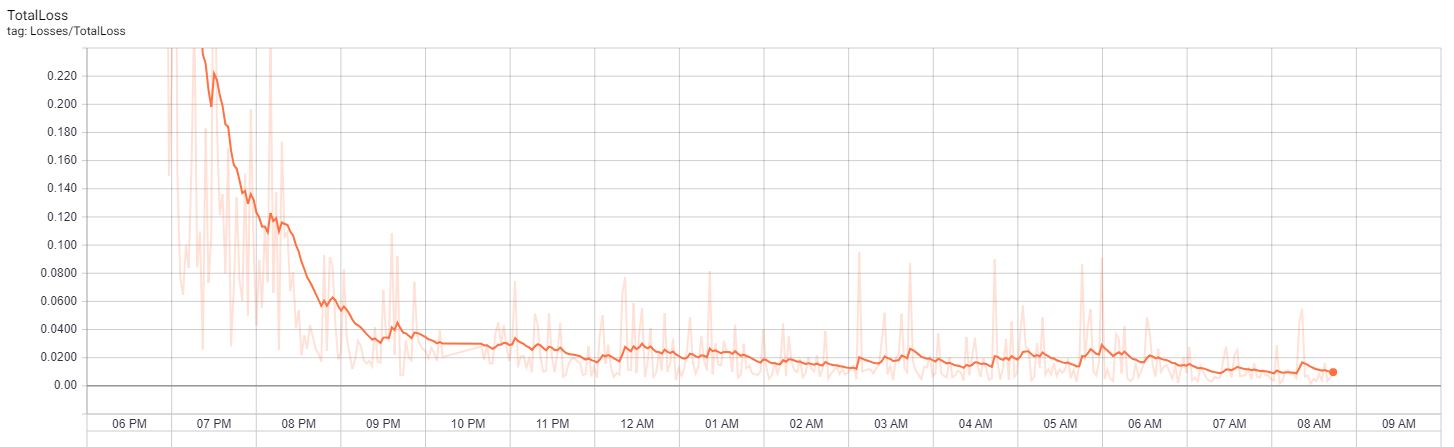
\includegraphics[scale=0.4]{Sources/loss_graph_200000.jpg}
	\caption{Loss Graph des umtrainierten inceptionV2}
	\label{img:loss_graph_200000}
\end{figure}

Der 'Loss' stellt dabei keine Prozentangabe dar, sondern ist eine Zusammenfassung der Fehler, die für jedes Beispiel in Trainings- oder Validierungssätzen gemacht wurden. Je kleiner der 'Loss dabei ist, desto höher ist die Wahrscheinlichkeit. Um die Grafik zu veranschaulichen, wurden kurzfristige Schwankungen geglättet. Zu beginn wird festgestellt, das die ersten 4 Stunden des Trainings den größten fortschritt aufweisen. In dieser Zeit, ist der 'Loss' von anfangs 2.0 auf 0.05 gesunken. Dabei wurden rund 60.000 Trainingseinheiten durchlaufen.\\
Die ersten Testergebnisse sehen gut aus. Alle beinhaltenden Objekte konnten erkannt und zugewiesen werden. Diese wurden auch mit einer hohen Wahrscheinlichkeit identifiziert. Lediglich bei der 'Orangensaft - Packung' hat das Netz einen Fehler gemacht. Diese wurde als Milch erkannt und das auch mit einer recht hohen Wahrscheinlichkeit. Zurückzuführen wäre das durch die hohe Ähnlichkeit der Formen.
\\

\begin{figure}
    [h]
	\centering
	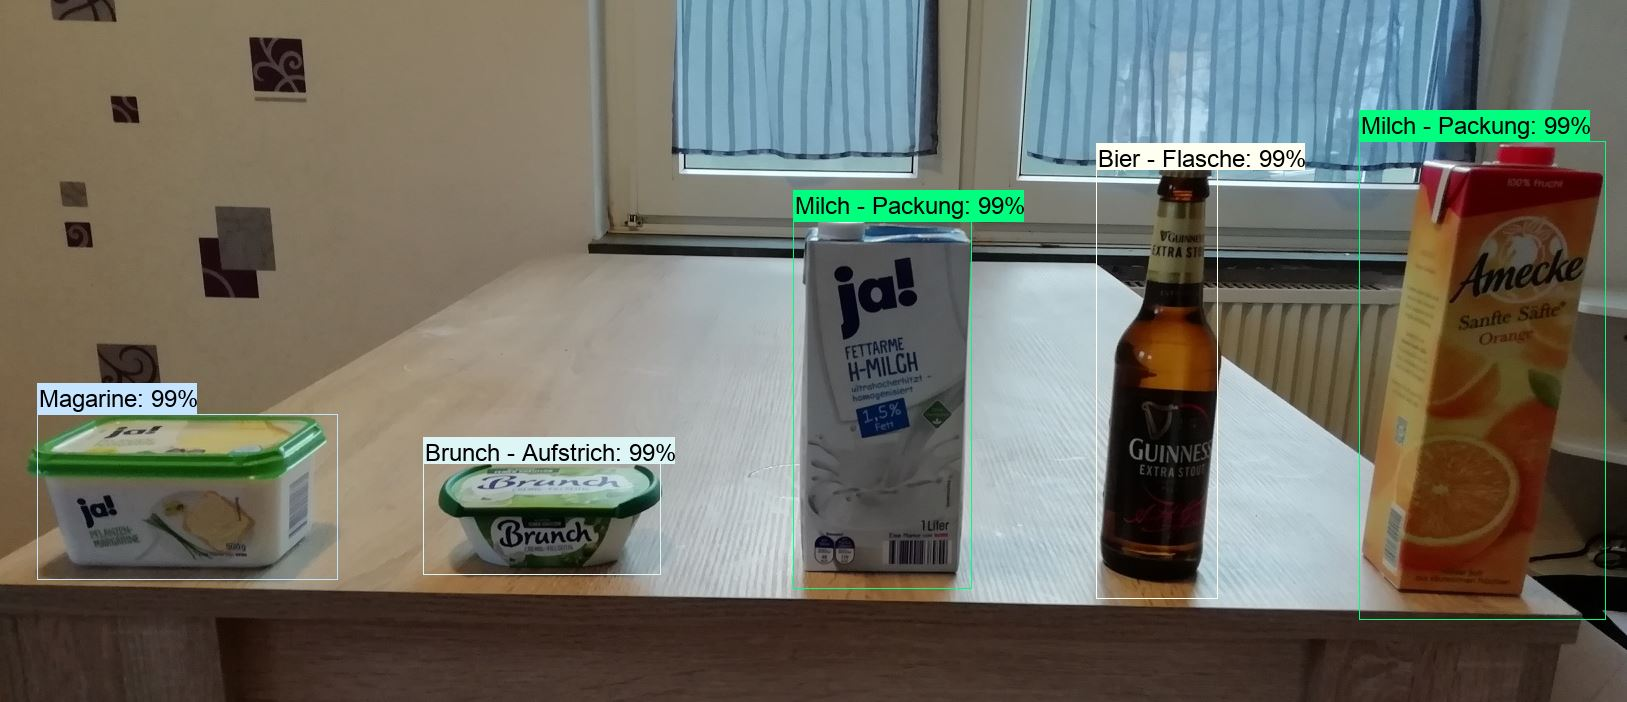
\includegraphics[scale=0.3]{Sources/Erster_Test.jpg}
	\caption{Erster Test des Neuronalen Netzes}
	\label{img:TestNN}
\end{figure}

Aus diesem Grund, soll überprüft werden, ob beim aufsetzen des Neuronalen Netzes Fehler gemacht wurden. Außerdem soll ein weiteres Vor-trainiertes Netze mit dem Datensatz getestet werden, Genauigkeit untereinander zu vergleichen. Das dafür ausgewählte Netz ist das faster\_rcnn\_resnet101\_coco. Dieses Modelle wurden aus der Tabelle? ausgewählt, da die mittlere durchschnittliche Genauigkeit.
\\
\\
Das zweite Modell welches trainiert wurde ist das faster\_rcnn\_resnet101\_coco mit einer mAP von 32 dafür ist es aber auch wesentlich langsamer. Für einen Trainingsdurchlauf benötigt das Modell mit rund 600ms im durchschnitt, mehr als doppelt so lange wie das faster\_rcnn\_inception\_v2\_coco. Es benötigt dafür aber auch nur die Hälfte an Durchläufen, um eine ähnlich niedrigen 'Loss' zu erreichen.\\ 

\begin{figure}
    [h]
	\centering
	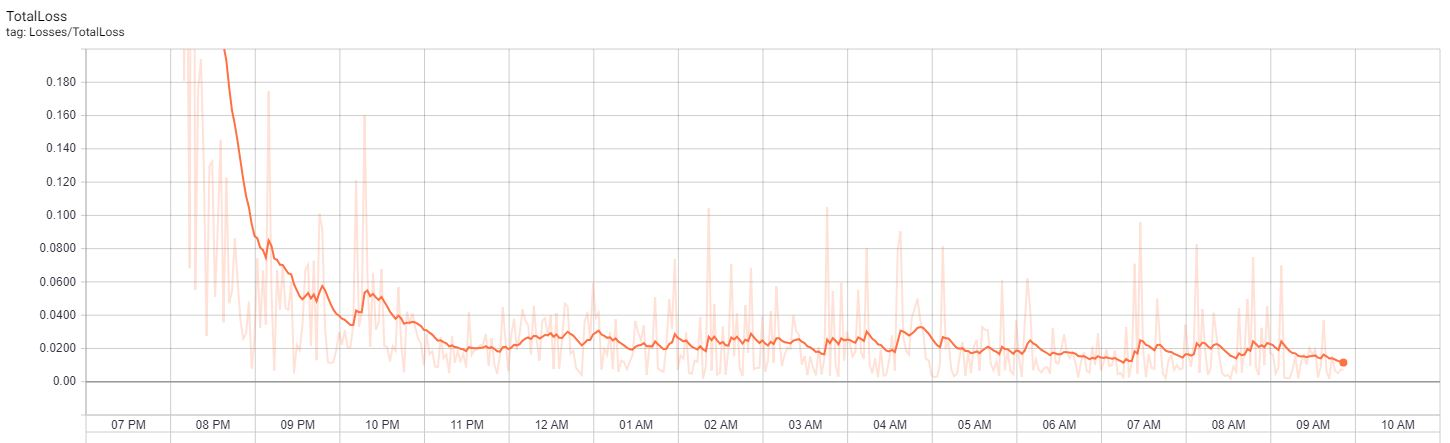
\includegraphics[scale=0.4]{Sources/loss_graph_resnet101.jpg}
	\vspace{0.5 cm}
	\caption{Loss Graph des umtrainierten resnet101}
	\label{img:loss_graph_resnet101}
\end{figure}

Testergebnisse der einzelnen Klassen zeigen auch das die Genauigkeit besser ist. Der Orangensaft welcher nicht identifiziert wurde, konnte jetzt erreicht werden. Dabei gab es wiederum das Problem das dieser je nach Winkel nicht immer richtig eingeordnet wurde. Um die Stabilität der ausgaben weiter zu erhöhen, sollen die Trainingsdaten weiter angehoben werden und das letzte Modell welches die höchste mAP hat soll auf den Datensatz trainiert werden.\\
\\
Weitere Test mit dem Trainierten Netz haben ergeben, das die Erkennung der Orangensaft Packung funktioniert, solange das Bild und die Oberflächen der Objekte nicht zu dunkel werden. Das Bild (Bild) zeigt alle Trainierten Objekte mit welchen das Modell faster\_rcnn\_resnet101\_coco trainiert wurde. Hier kann man erkennen das alle Klassen richtig zugeordnet werden konnten.

\begin{figure}
    [h]
	\centering
	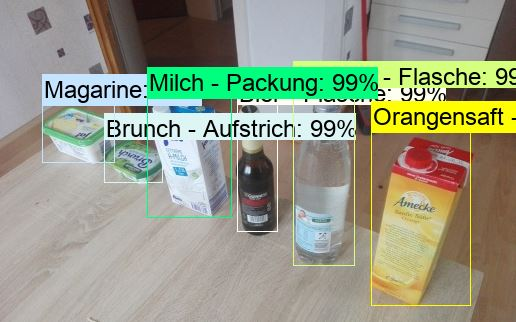
\includegraphics[scale=0.5]{Sources/final_detection.jpg}
	\vspace{0.3 cm}
	\caption{Objekt erkennung des optimierten resnet101}
	\label{img:loss_graph_resnet101}
\end{figure}

Abgesehen von den schwächen in der Erkennung ähnlicher Objekte hat das generieren eines Neuronalen Netzes Funktioniert. Im nächsten Kapitel sollen die Ergebnisse des Projektes, mit den Anforderungen verglichen und ausgewertet werden.

\newpage

\section{Fazit}
Wie im vorherigen Kapitel beschrieben, hat die Entwicklung eines Künstlichen Neuronalen Netzes gut funktioniert. Lediglich bei ziemlich ähnlichen Objekten, gab es Probleme mit der richtigen Identifizierung. Um ein finales Fazit geben zu können soll in diesem Kapitel auf die Anforderungen eingegangen werden, welche zu Beginn des Projektes festgelegt wurden.\\

\subsection{Bewertung durch Anforderungen}

Die ersten Zwei funktionalen Anforderungen konnten erfüllt werden. Lediglich die Genauigkeit konnte zunächst nicht zu voller Zufriedenheit erfüllt werden. Die meisten Objekte können bei schlechteren Bild- und Lichtverhältnissen erkannt werden, lediglich bei zu ähnlichen Objekten kann die Erkennung fehlerhaft sein, wie man bei der Milch und dem Orangensaft beobachten kann. Mit mehreren Trainingsdaten und einer Licht Korrektur könnte dies allerdings verbessert werden.\\
\\
Die organisationalen Anforderungen konnten auch zum Großteil erfüllt werden. Klassen können unkompliziert erweitert werden, indem Testdaten der gewünschten Klasse Generiert und gelabelt werden. Das trainieren und ausführen des Neuronalen Netzes ist zwar im Moment nicht mit einer Datei ausführbar, aber die notwendigen schritte sind nicht aufwendig. Die Installation aller Notwendigen Module und Bibliotheken kann durch die Eingabeaufforderung oder der shell ausgeführt werden. Lediglich für Anaconda muss man eine manuelle Installation durchführen. Das Netz kann auf jedem Endgerät mit der benötigten Entwicklungsumgebung betrieben werden. Für mobile Endgeräte ist das Netz jedoch wegen der benötigten Rechenleistung nicht geeignet.\\
\\
Bei den qualitativen Anforderungen kann man nicht jede erfüllen, weil je höher die Genauigkeit des Netzes ist, desto länger benötigt es um ein Bild auszuwerten. Umgekehrt sinkt die Genauigkeit umso schnelle das Netz arbeitet. Es wurde also darauf geachtet das es bei beiden Punkten solide Ergebnisse erzielt. Der Schwerpunkt lag aber auf der Genauigkeit des Netzes. Leicht verdeckte Objekte können auch bis zu einem Gewissen Punkt erkannt und richtig zugeordnet werden. Die Genauigkeit kann beispielsweise, durch mehrere Trainingsdaten erhöht werden.\\

\subsection{Bewertung der Netze}
Das Neuronale Netz funktioniert größtenteils wie gewollt, nur bei zwei Klassen kann nicht immer Korrekt unterschieden werden. Das liegt hauptsächlich an der hohen Ähnlichkeit der zwei Objekte. Die Genauigkeit könnte durch eine höhere Anzahl an Trainings und Testdaten verbessert werden. Außerdem könnte eine Angleichung der Lichtverhältnisse per Bildverarbeitung dafür sorgen, dass die Genauigkeit des Netzes steigt. Zwischen den getesteten Modellen wurde festgestellt, das die Übereinstimmung der Objekte einen wesentlichen unterschied in der Genauigkeit aufweisen, sodass eine etwas höhere Antwortzeit für den Verwendungszweck kein großes Problem darstellt.\\
\\
Abschließend, kann das Projekt als Erfolgreich angesehen werden, mit kleinen Optimierungen.

\section{Aussicht}
Die Entwicklung eines neuronalen Netzwerkes hat gezeigt, das es Möglich ist den Inhalt Regal-Systeme mit Hilfe von Objekterkennung zu Identifizieren. Dabei ist aber auch aufgefallen, das mehr Trainingdaten benötigt werden je Ähnlicher sich die Klassen sind. Das bedeutet das für das geplante System eine große Anzahl an Trainingsdaten generiert werden müssen. Grundsätzlich ist es aber möglich mit den Ergebnissen weiter Arbeiten zu können.\\
\\
Für das Geplante System wären bis auf die Optimierung des Künstlichen neuronalen Netzes, die Systemschnittstellen welche zum einen das Bild vom Regal aufnimmt, verarbeitet und an das neuronale Netz weiter leitet und zum anderen müssen die Informationen der Bilderkennung an eine Datenbank übergeben werden, welche den Inhalt des Regals speichert. Darüber hinaus müsste eine Anwendung entwickelt werden, mit welcher der Benutzer den Inhalt des Regals managen kann.\\
\\
Die Optimierung soll aber Für die Nächsten Schritte im Vordergrund stehen. Für die anstehende Bachelorarbeit, soll die Verbesserung des Neuronalen Netzes im Vordergrund stehen. dabei gibt es drei wichtige Punkte welche behandelt werden müssen. Zum einen soll die Genauigkeit der Identifizierung bei ähnlichen Objekten erhöht werden. Außerdem sollen Bildaufnahmen so verarbeitet werden, das Lichtverhältnisse gleich sind oder eine Veränderung dieser Keinen Einfluss auf die Ergebnisse haben. Zusätzlich soll die Auswirkung schlechter Bildverhältnisse ermittelt und Verbessert werden.
   
  
  
\end{document}

